%%%%%%%%%%%%%%%%%%%%%%%%%%  phdsymp_sample2e.tex %%%%%%%%%%%%%%%%%%%%%%%%%%%%%%
%% changes for phdsymp.cls marked with !PN
%% except all occ. of phdsymp.sty changed phdsymp.cls
%%%%%%%%%%                                                       %%%%%%%%%%%%%
%%%%%%%%%%    More information: see the header of phdsymp.cls   %%%%%%%%%%%%%
%%%%%%%%%%                                                       %%%%%%%%%%%%%
%%%%%%%%%%%%%%%%%%%%%%%%%%%%%%%%%%%%%%%%%%%%%%%%%%%%%%%%%%%%%%%%%%%%%%%%%%%%%%%


%\documentclass[10pt]{phdsymp} %!PN
\documentclass[twocolumn]{phdsymp} %!PN
%\documentclass[12pt,draft]{phdsymp} %!PN
%\documentstyle[twocolumn]{phdsymp}
%\documentstyle[12pt,twoside,draft]{phdsymp}
%\documentstyle[9pt,twocolumn,technote,twoside]{phdsymp}

\usepackage[english]{babel}       % Voor nederlandstalige hyphenatie (woordsplitsing)
\usepackage{tikz}
\usepackage{url}
\usepackage{graphicx}
\usepackage[tablename=Tab.]{caption}
\usepackage{subcaption}
\captionsetup{compatibility=false}
\usepackage[acronym,xindy,style=super, nonumberlist]{glossaries}
\graphicspath{{figuren/}}               % De plaats waar latex zijn figuren gaat halen.
\usepackage{booktabs}
\usepackage{times}
\usepackage{amsfonts}
\usepackage{bbm}
\usepackage{amsmath,scalefnt}

\usetikzlibrary{automata}
\usetikzlibrary{decorations.pathreplacing}
\usetikzlibrary{shapes, arrows, shadows, positioning, backgrounds}
\usetikzlibrary{trees}
\tikzstyle{state}=[shape=circle,draw=black!50,scale=2.0]
\tikzstyle{staterect}=[shape=rectangle,draw=black!50]
\tikzstyle{state_small}=[shape=circle,draw=black!50,scale=1.5]
\tikzstyle{state2}=[minimum width=8pt,shape=circle,draw=blue!50,fill=blue!20]
\tikzstyle{observation}=[shape=rectangle,draw=orange!50,fill=orange!20]
\tikzstyle{lightedge}=[<-,dotted]
\tikzstyle{mainstate}=[state,thick]
\tikzstyle{mainedge}=[<-,thick]

\hyphenation{si-mu-la-ted re-a-lis-tic packets really in-clu-ding}

\def\BibTeX{{\rm B\kern-.05em{\sc i\kern-.025em b}\kern-.08em
    T\kern-.1667em\lower.7ex\hbox{E}\kern-.125emX}}

\newtheorem{theorem}{Theorem}

\makeglossaries
\newacronym{drl}{DRL}{deep reinforcement learning}
\newacronym{sl}{SL}{supervised learning}
\newacronym{td}{TD}{temporal difference}
\newacronym{ai}{AI}{artificial intelligence}
\newacronym{sota}{SOTA}{state of the art}
\newacronym{rl}{RL}{reinforcement learning}
\newacronym{cnn}{CNN}{convolutional neural network}
\newacronym{nn}{NN}{neural network}
\newacronym{fnn}{FNN}{feedforward neural network}
\newacronym{mdp}{MDP}{Markov decision process}
\newacronym{mse}{MSE}{mean squared error}
\newacronym{sgd}{SGD}{stochastic gradient descent}
\newacronym{pv}{PV}{principal variation}
\newacronym{fcn}{FCN}{fully connected network}
\newacronym{dtm}{DTM}{depth to mate}
\newacronym{wdl}{WDL}{win draw loss}
\newacronym{krk}{KRK}{king rook king}
\newacronym{kqk}{KQK}{king queen king}
\newacronym{wcr}{WCR}{win conversion rate}
\newacronym{we}{WE}{win efficiency}
\newacronym{lhs}{LHS}{loss holding score}
\newacronym{relu}{ReLU}{rectifier linear unit}
\captionsetup{tablename=Tab.}
\begin{document}

\title{Teaching Computers to Play Chess with Deep Reinforcement Learning} %!PN

\author{Dorian Van den Heede}

\supervisor{Francis wyffels, Jeroen Burms, Joni Dambre}

\maketitle

\begin{abstract}
Chess computers have reached a superhuman level at playing chess by combining tree search with the incorporation of heuristics obtained with expert knowledge into the value function when evaluating board positions. Although these approaches add a big amount of tactical knowledge, they do not tackle the problem of effectively solving chess, a deterministic game. We try to set the first stone by solving relatively simple chess endgames from a human point of view with \gls{drl}. The proposed \gls{drl} algorithm consists of 2 main components: (i) self play (ii) translating the collected data in phase (i) to a \gls{sl} framework with deep learning. In light of this, we present a novel \gls{td} learning algorithm, TD-Stem($\lambda$), and compare it with the state of the art, TD-Leaf($\lambda$).
\end{abstract}

\begin{keywords}
Chess, deep reinforcement learning, TD-learning
\end{keywords}

\section{Introduction}
\PARstart{I}{n} the early 50s, scientists like Shannon and Turing were already musing about how a machine would be able to play chess autonomously \cite{shannon,turing}. The enormous complexity ($\sim 10^{120}$ different states) combined with its popularity and rich history made it the holy grail of \gls{ai} research in the second half of the $20^{\textnormal{th}}$ century. Research attained its peak in 1997 when \textit{Deep Blue} succeeded at winning a duel with the human world champion at that time, \textit{Gary Kasparov} \cite{deepblue}. Conventional chess computers now attain a superhuman level.\\
Current \gls{sota} engines use a combination of deep search trees with expert knowledge heuristics to evaluate positions at leaf nodes (\textit{Komodo},\textit{Stockfish} and \textit{Houdini} at time of writing) \cite{sota}. Furthermore, the search is heavily optimized as an attempt to reduce the influence of the exponentially increasing complexity when looking more moves ahead. The height of the search tree is the most crucial factor for the performance of an engine. These observations lead to the following shortcomings: (i) the strategic strength is entirely based on the heuristical evaluation at leaf nodes, which is humanly biased and suboptimal as a consequence (ii) conventional play by engines is very tactical as the reached depth is the most important variable for performance, resulting in a lack of intuitive game play (iii) as current engines mostly rely on human insight, they do not take steps at objectively solving the game, but more at how to beat humans with their advantage in calculation power.\\
These downsides could eventually be solved by looking at the game in a primitive and unbiased viewpoint and using a combination of self play with supervised machine learning in a \gls{rl} framework. As a first step we have implemented a deep learning architecture where we use a novel TD-learning variant in combination with neural networks being fed by positions represented as bitboards.\\
This paper is organized as follows. In section \ref{sec:relwork} a brief overview of previous research in this domain is given. Section \ref{sec:drl} introduces the used \gls{drl} framework after which we focus on how different modifications of the well known TD($\lambda$) algorithm may unite strategic and tactical information into the value function in section \ref{sec:td}. The value function itself is discussed in \ref{sec:nn}. We compare our novel algorithm with the \gls{sota} TD-learning algorithm for chess in section \ref{sec:res} and form an appropriate conclusion in section \ref{sec:con}.

\section{Related Work}
\label{sec:relwork}
Already in 1959, a TD-learning algorithm was used to create a simplistic checkers program \cite{samuel}. The first real success story of using TD-learning (arguably for \gls{rl} in general) and \Gls{nn} for value function approximation in boardgames was \textit{Tesouro}'s backgammon program \textit{TD-Gammon} with a simple fully connected \gls{fnn} architecture learned by incremental TD($\lambda$) updates \cite{tesauro}. One interesting consequence of \textit{TD-Gammon} is its major influence on strategic game play of humans in backgammon today. As chess is a game where tactics seem to have the upper hand over strategic thinking, game tree search is used to calculate the temporal difference updates in TD-Leaf($\lambda$) proposed by \textit{Baxter} et al. The chess software \textit{KnightCap} that came out of it used linear expert knowledge board features for function approximation and had learned to play chess up until master level by playing on a chess server. The same method was used in combination with a two layer \gls{nn} initialized with biased piece value knowledge in \textit{Giraffe} to reach grandmaster level, effectively proving the potential strength of TD-learning methods with search at a limited depth \cite{giraffe}.  Veness et al.went even further and stored as much information from game tree search during self play as possible in \textit{Meep} \cite{meep}.\\
The potential of using millions of database games between experts to learn to play chess has been exploited in \textit{DeepChess} \cite{deepchess}.\\

In \gls{rl} research concerning other games, \glspl{cnn} have already been proven its worth. A lot of research has been undertaken to Atari video games, which makes sense as \glspl{cnn} were originally designed for computer vision tasks \cite{atari}. The current \gls{sota} is a dual network learning the advantage function with double deep Q-learning \cite{dddqn}. The first successful application of \Gls{cnn} into boardgames is \textit{AlphaGo}, which is the first \textit{Go} program to beat a player with the highest possible rating \cite{alphago}.   

\section{Deep Reinforcement Learning Framework for Chess}
\label{sec:drl}
Our system consists out of two main components, namely self play and the incorporation of newly seen data into the system. These two phases are performed iteratively. In section \ref{sec:rl} chess is formulated as an \gls{rl} framework. The system updates are explained with the help of an \gls{sl} framework in section \ref{sec:sl}.

\subsection{Reinforcement Learning}
\label{sec:rl}
In \gls{rl}, agents are released in an environment where they have to find out by exploration which actions generate the best cumulative rewards. In this case, the board is the environment and white and black are the agents. When one player succeeds at mating the opponent, a positive reward is provided.\\
To this cause, we have to model chess as a deterministic \gls{mdp} $\mathcal{M}=(\mathcal{S},\mathcal{A}$ $,r,\gamma)$ with \cite{rl}
\begin{itemize}
\item $\mathcal{S}$: state space containing all possible board positions
\item $\mathcal{A}$: action space, which holds all possible actions. ${\mathcal{A}}_s$ is the set of playable moves in board position $s\in \mathcal{S}$.
\item $r_A:\mathcal{S} \times \mathcal{A}_{\mathcal{S}} \mapsto \mathbb{R}$ is the immediate reward function for player $A\in\{W,B\}$ (white or black).
\item $\gamma \in \mathbb{R}$ $ \cap \left[0,1\right]$: the discount factor
\end{itemize}
The chess environment is episodical, meaning it has terminal states (checkmate, stalemate, ...). An episode is represented with its history from whites perspective\[H=\left\{(s_0,a_0,r_1),(s_1,a_1,r_2), \dotso , (s_{T-1},a_{T-1},r_{T})\right\}\]
where we assume $a_i\in {\mathcal{A}}_{s_i}$ $, \forall i \in 0,\cdots,T-1$, i.e.only legal moves according to the rules of chess can be made in the environment, and $r_{i+1}=r_W(s_{i},a_{i})$.\\
The history is used for the calculation of the return of a certain state in an episode, which is defined as the exponentially discounted sum of the observed rewards: $R_{t}=\sum_{t'=t}^{T-1}\gamma^t r_{t'+1}$. The return is the quantity agents (players) acting on the environment try to optimize. As chess is a game with the zero-sum property, $r_W(s_t,a_t)=-r_B(s_t,a_t)$, the optimization goals for white and black are maximizing and minimizing $R$ respectively (white is generally called the max-player, black the min-player). Consequently, it is the goal of the agents to arrive in positions which have the most optimized expected return, as this will in general optimize their future rewards. This is represented by the value function:
\begin{align}
V(s_t) &= \textnormal{E}\left[R_t|s\right] \\
	 &= \textnormal{E}\left[\sum_{t'=t}^{T-1}\gamma^t r_{t'+1}|s\right]
\end{align} 

Furthermore, the chess environment is simplified as follows:
\begin{itemize}
\item $\gamma=1$
\item $r_W(s_t,a_t) = \begin{cases} 
   1 & \text{if } s_{t+1} \textnormal{ is checkmate}\\
   0 &  \textnormal{else} \\
  \end{cases}$
\end{itemize}

This allows the rewards to be transposed to the final outcome $z_H$ of an episode with history $H$:
\begin{align}
z_H&=r_T \\
&=r_W(s_{T-1},a_{T-1})
\end{align}
As rewards are only accounted at the terminal state, the expression for the value function is reduced to the expected value of the final outcome $z$
\begin{equation}
V(s) = \textnormal{E}\left[z|s\right]
\end{equation}
The impossibility to store $V(s)$ for every state speaks for itself, which is why it is represented with a function approximation method (section \ref{sec:nn}). How to update $V(s)$ with \gls{sl} is the topic of section \ref{sec:sl}.\\

The optimal policy given $V^*(s)$ is simply making the greedy choice (define the state successor function $\Sigma(s_t,a_t)=s_{t+1}$ yielding the next board after making action $a_t$ on state $s_t$)
\begin{equation}
a_{t}^*=\textnormal{arg} \max_{a\in{\mathcal{A}}_{s_t}} V^*(\Sigma(s_t,a))
\end{equation}
However, due to the tactical nature of chess it is very hard to obtain a good policy by only looking one ply ahead. That is why here and in chess in general some sort of optimized minimax search is performed. This consists of building a tree up to a depth $d$ and evaluating the leaf nodes. For the minimax policy it is then assumed that both max- and min-player are playing the best move with respect to the leaf node evaluations at depth $d$. The path in the tree following the minimax policy is called the \gls{pv}. \\
Because of the exploration-exploitation dilemma, an over time decaying $\epsilon$-greedy policy is applied during self play \cite{rl}.

\subsection{Supervised Learning}
\label{sec:sl}
In \gls{sl}, the task is to infer a function (in our case $V(s)$, making this a regression problem) that generalizes labeled training data. 
Supposing $V_\theta$ is differentiable with respect to its tunable parameters $\theta$, an obvious choice for the learning algorithm in an \gls{sl} context is \gls{sgd} with the \gls{mse} as loss function: $L_\theta(s,\hat{z})=\left(V_\theta(s)-\hat{z}\right)^2$. The total loss over all $N$ encountered states in an iteration of self play is then $L_\theta=\frac{1}{N}\sum_s L_\theta(s,\hat{z})$. The parameters are updated in the direction of steepest descent with step size $\alpha$ by calculation of the gradient of the loss function:
\begin{equation}
\theta \leftarrow \theta-\alpha\nabla L_\theta
\label{eq:blackbox}
\end{equation}
Every episode individually corresponds to the update
\begin{equation}
\theta\leftarrow \theta-\frac{\alpha}{T}\sum_{t=0}^{T-1}\left(\hat{z}_t-V_\theta(s_t)\right)\nabla V_\theta(s_t)
\label{eq:insight}
\end{equation}
Both update rules are equivalent, but equation \ref{eq:insight} gives more insight regarding the direction we are optimizing to. Equation \ref{eq:blackbox} is more a black box, ideal for software libraries only needing a set of $(s,\hat{z})$ tuples to perform (mini-batch) \gls{sgd}.\\

We chose $V(s)$ to be a neural network (\gls{fnn} or \gls{cnn}) because of its capability to learn complex patterns and features from raw data with \gls{sgd} through the backpropagation for differentiation. As a main constraint in this research is to be completely unbiased, this is a necessary condition.\\

All that remains to be found are appropriate training samples $(s,\hat{z})$ given the histories of simulated episodes during self play, where $\hat{z}$ is preferably the best possible estimation for the true outcome. In the presented system, $\hat{z}$ is calculated with game tree search TD-learning methods, presented in section \ref{sec:td}.

\section{TD-Learning}
\label{sec:td}
TD algorithms are ideal in an \gls{sl} framework, because of its natural embedding of the optimization of the \gls{mse} cost function in its update rule \cite{rlalg}. An additional advantage specific to chess is that no policy needs to be learned to make it work, which would be hard considering the diverse possibilities of legal moves in chess positions.\\
The core idea of TD-learning is to update the weights of the value function in the direction of what is supposed to be a better estimate found out one time step later. The observed error is called the temporal difference
\begin{equation}
\delta_t=V_\theta(s_{t+1})-V_\theta(s_t)
\end{equation}
where we suppose $V_\theta(s_T)=z_H$ from now on if $s_T$ is a terminal state. The episodical update in pure TD-learning (also called TD(0)) is
\begin{equation}
\theta\leftarrow \theta-\frac{\alpha}{T}\sum_{t=0}^{T-1}\nabla V_\theta(s_t)\delta_t
\label{eq:td0}
\end{equation}

\subsection{TD-($\lambda$)}
By introducing an additional exponential weight decay parameter $0\leq\lambda\leq1$ credit can be given to more distant states. The resulting update after the simulation of an episode corresponds to
\begin{equation}
\theta\leftarrow \theta-\frac{\alpha}{T}\sum_{t=0}^{T}\nabla V_\theta(s_t)\sum_{n=t}^{T-1}\lambda^{n-t}\delta_t
\label{eq:tdlambda}
\end{equation}
From equations \ref{eq:insight} and \ref{eq:tdlambda} we derive a formula to set the target values $\hat{z}_t$ for a \gls{sl} framework which can be learned with (mini-batch) \gls{sgd} on bigger datasets after simulating a whole iteration of episodes:
\begin{equation}
\hat{z}_t=V_\theta(s_t)+\sum_{n=t}^{T-1}\lambda^{n-t}\delta_t
\label{eq:target}
\end{equation}

\subsection{TD-Leaf($\lambda$)}
With the understanding of the machinery in TD($\lambda$), we have weaponed ourselves to extend the algorithm to include game tree search. Call $l(s_t,d)$ the node at depth d in the \gls{pv}. TD-Leafs goal is then to modify the value function of $l(s_t,d)$ to $l(s_{t+1},d)$. Hence, the equations can be written out as
\begin{equation}
\delta_t=V_\theta(l(s_{t+1},d))-V_\theta(l(s_t,d)) 
\label{tdl}
\end{equation}
\begin{equation}
\theta\leftarrow\theta-\frac{\alpha}{T}\sum_{t=0}^{T}\nabla V_\theta(l(s_t,d))\sum_{n=t}^{T-1}\lambda^{n-t}\delta_t
\end{equation}
Instead of updating the encountered state as in TD($\lambda$), the leaf nodes are updated, ensuring the collected data to be less correlated. Furthermore, minimax search is included in the algorithm.\\
A downside to this algorithm is the influence of the outcome of an episode to the update of a state which was not part of that episode, as it could be that the updated leaf state was only encountered in the minimax search and not at all in the true simulation. We will call this an update into the direction of 'wrong belief', credit has not been given where it is due.

\subsection{TD-Stem($\lambda$)}
The novel proposal is to include depth information gathered from experience into the value function. Although this may have the issue of including more noise into the value function and making it less smooth complicating \gls{sgd}, it could speed up training by self play as depth information is propagated faster from terminal positions. \\
The way this would work is to update the static evaluation function of the encountered state to the temporal difference between the successive leafs at the \Gls{pv} (equation \ref{tdl}). The target values for the encountered states are given by equation \ref{eq:target}.\\
A visual comparison between the algorithms is given in figure \ref{fig:algs}.

\begin{figure}
    \centering
    \begin{subfigure}{0.4\textwidth}
        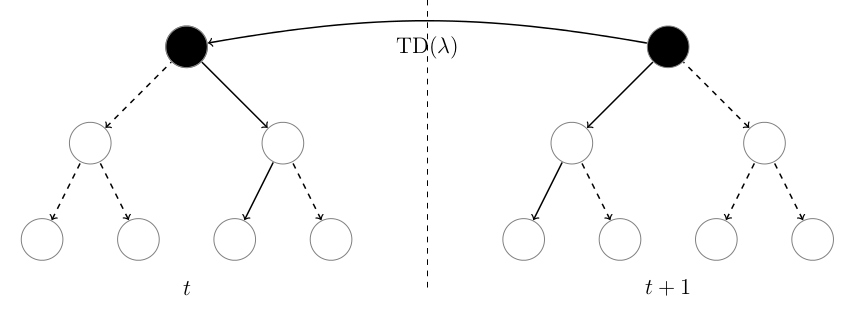
\includegraphics[scale=0.25]{tdlambda}
    \end{subfigure}
    \begin{subfigure}{0.4\textwidth}
        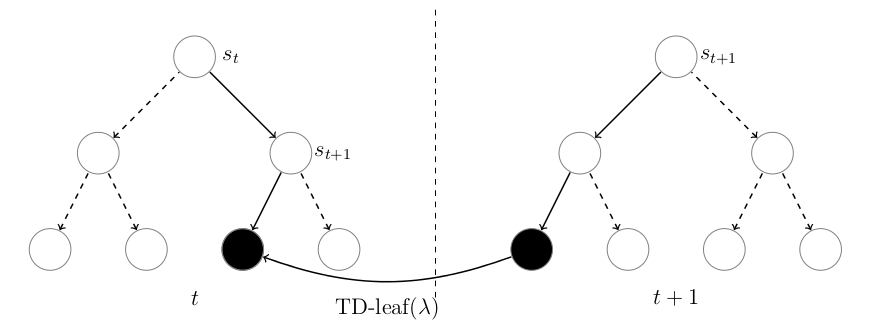
\includegraphics[trim={0.25cm 0cm 0 0cm},clip,scale=0.25]{tdl}
    \end{subfigure}
    \begin{subfigure}{0.4\textwidth}
        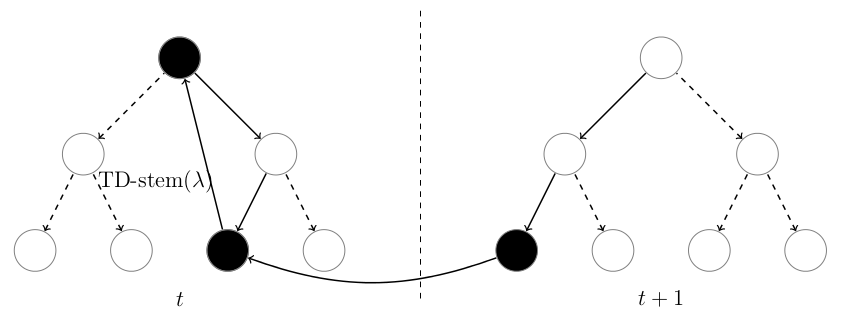
\includegraphics[trim={0cm 0cm 0.5cm 0cm},clip,scale=0.25]{tds}
    \end{subfigure}
    \caption{Comparison between the 3 discussed TD-learning algorithms, the \Gls{pv} are indicated with solid edges. In classical TD-learning the updates are between successive states. TD-leaf updates are between successive leaf nodes and in TD-stem both ideas are combined. }\label{fig:algs}
\end{figure}


\section{Network Architecture}
\label{sec:nn}
In conventional chess engines, the heuristic evaluation function is linear, but also reinforcement learning chess programs often use a linear value function \cite{knightcap,meep}. In this dissertation, we switched gears and used a neural network model instead, as they have the ability to model a larger range of functions and extract additional features from the data. Additionally, they perform quite good in practice although they do not necessarily converge under TD algorithms \cite{convergence}. Here, there has been experimented with a \gls{cnn} architecture using raw image planes as input, which is a first to our best knowledge. The activation function between all hidden units is an ordinary \gls{relu} and the weights are initialized with the tips given by Bengio et al. \cite{init}.\\

Chess boards are separated in two sets of features:
\begin{itemize}
\item bitboards: raw image planes (8x8)
\item global features: objective observations about the board 
\end{itemize}
An example of how to extract bitboards from a chess position is shown in table \ref{tab:feat}, where the chess board in figure \ref{fig:diagram} is vectorized. Feature maps are extracted from the binary image planes which are fed into a \gls{cnn}. The global features come together with a flattened version of the feature maps at the output of the final convolutional layer in a final \gls{fcn} in order to obtain the static evaluation.

\begin{figure}
\centering
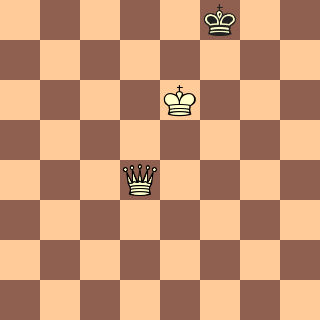
\includegraphics[scale=0.5]{diagram}
\caption{}
\label{fig:diagram}
\end{figure}

\begin{table}[]
\caption{8 Bitboards corresponding to the chess position in figure \ref{fig:diagram}. Piece maps indicate the cells where pieces reside. Mobility maps show where pieces can go to.}
\label{tab:feat}
\centering
\begin{tabular}{c c c}
\hline
\textbf{piece} & \textbf{piece map} & \textbf{mobility map}  \\
\hline
&&\\

\includegraphics[scale=0.5]{pieces/K} & 
$\begin{smallmatrix}0&0&0&0&0&0&0&0\\0&0&0&0&0&0&0&0\\0&0&0&0&1&0&0&0\\0&0&0&0&0&0&0&0\\0&0&0&0&0&0&0&0\\0&0&0&0&0&0&0&0\\0&0&0&0&0&0&0&0\\0&0&0&0&0&0&0&0\end{smallmatrix}$
&
$\begin{smallmatrix}0&0&0&0&0&0&0&0\\0&0&0&1&0&0&0&0\\0&0&0&1&0&1&0&0\\0&0&0&1&1&1&0&0\\0&0&0&0&0&0&0&0\\0&0&0&0&0&0&0&0\\0&0&0&0&0&0&0&0\\0&0&0&0&0&0&0&0\end{smallmatrix}$
\\&&\\

\includegraphics[scale=0.5]{pieces/Q} & 
$\begin{smallmatrix}0&0&0&0&0&0&0&0\\0&0&0&0&0&0&0&0\\0&0&0&0&0&0&0&0\\0&0&0&0&0&0&0&0\\0&0&0&1&0&0&0&0\\0&0&0&0&0&0&0&0\\0&0&0&0&0&0&0&0\\0&0&0&0&0&0&0&0\end{smallmatrix}$
&
$\begin{smallmatrix}0&0&0&1&0&0&0&1\\1&0&0&1&0&0&1&0\\0&1&0&1&0&1&0&0\\0&0&1&1&1&0&0&0\\1&1&1&0&1&1&1&1\\0&0&1&1&1&0&0&0\\0&1&0&1&0&1&0&0\\1&0&0&1&0&0&1&0\end{smallmatrix}$
\\&&\\

\includegraphics[scale=0.5]{pieces/k} &
$\begin{smallmatrix}0&0&0&0&0&1&0&0\\0&0&0&0&0&0&0&0\\0&0&0&0&0&0&0&0\\0&0&0&0&0&0&0&0\\0&0&0&0&0&0&0&0\\0&0&0&0&0&0&0&0\\0&0&0&0&0&0&0&0\\0&0&0&0&0&0&0&0\end{smallmatrix}$
 & 
$\begin{smallmatrix}0&0&0&0&1&0&1&0\\0&0&0&0&0&0&0&0\\0&0&0&0&0&0&0&0\\0&0&0&0&0&0&0&0\\0&0&0&0&0&0&0&0\\0&0&0&0&0&0&0&0\\0&0&0&0&0&0&0&0\\0&0&0&0&0&0&0&0\end{smallmatrix}$
\\&&\\ 
\includegraphics[scale=0.5]{pieces/q} &
$\begin{smallmatrix}0&0&0&0&0&0&0&0\\0&0&0&0&0&0&0&0\\0&0&0&0&0&0&0&0\\0&0&0&0&0&0&0&0\\0&0&0&0&0&0&0&0\\0&0&0&0&0&0&0&0\\0&0&0&0&0&0&0&0\\0&0&0&0&0&0&0&0\end{smallmatrix}$
&
$\begin{smallmatrix}0&0&0&0&0&0&0&0\\0&0&0&0&0&0&0&0\\0&0&0&0&0&0&0&0\\0&0&0&0&0&0&0&0\\0&0&0&0&0&0&0&0\\0&0&0&0&0&0&0&0\\0&0&0&0&0&0&0&0\\0&0&0&0&0&0&0&0\end{smallmatrix}$
\\&&\\
\hline
\end{tabular}
\end{table}


\section{Experiments}
\label{sec:res}
We performed two experiments on basic endgame problems by letting 2 agents with the same value function play episodes against each other starting from a random position sampled from a generated dataset and compared the final performances of TD-Leaf and TD-Stem by playing 2000 games against an optimal player making perfect moves after training. The optimality is obtained by probing a Gaviota tablebase, containing the exact \gls{dtm} and \gls{wdl} information \cite{tb}. We propose 3 metrics, the \gls{wcr}, \gls{we} and \gls{lhs} to assess the quality of a model: \textcolor{white}{Fabian}
\begin{align*}
\textnormal{WCR}&=\frac{\text{games model won}}{\text{games model should win}} \\
\textnormal{WE}&=\frac{\text{average DTM of won games}}{\text{average length of won games}}\\
\textnormal{LHS}&=\frac{\text{average length of lost games}}{\text{average DTM of lost games}}\\
\end{align*}

The complete simulation is performed through stages, which are manually controllable.
The process has been further optimized with the addition of hyper-parameters (see table \ref{tab:params_exp}), modifiable through stages. In table \ref{tab:stages} the configurations for the stages conducted in the experiments are laid out.

\begin{table}[]
\centering
\caption{Hyper-parameters modifiable in between stages.}
\label{tab:params_exp}
\begin{tabular}{rl}
\hline
$\lambda$    & Parameter for TD-learning methods                                                                                                        \\ 
$d_r$        & Depth at which immediate wins are sought                                                                                      \\ 
$d_V$        & Depth at which the value network is called                                                                                               \\ 
$f_\epsilon$ & \begin{tabular}[c]{@{}l@{}}Decay function for exploration parameter $\epsilon =f(i)$.\\  i increments every iteration.\end{tabular}      \\ 
$I$          & Number of iterations                                                                                                                     \\ 
$i_0$        & First iteration number, to initialize $\epsilon$ with the $f_\epsilon$                                                                   \\ 
$K$          & \begin{tabular}[c]{@{}l@{}}The number of states that are used to calculate the\\ $\lambda$-return from an episode\end{tabular}          \\ 
$M$          & The maximal amount of moves made in an episode                                                                                           \\ 
$N$          & How many games are played during an iteration                                                                                            \\ 
$R$          & \begin{tabular}[c]{@{}l@{}}The number of additional random moves played on the \\board position extracted from the dataset\end{tabular} \\ \hline
\end{tabular}
\end{table} 


\begin{table}[]
\centering
\caption{Hyper-parameters of the stages in the experiments}
\label{tab:stages}
\begin{tabular}{cc|rrrrrrr}
\textbf{Exp}&\textbf{Stage} & \textbf{$N$}  & \textbf{$I$} & \textbf{$d_V$} & \textbf{$\lambda$}& \textbf{$i_0$}&$K$ &$d_r$\\ \hline
& 1     & 5000 & 20  & 1     & 0.5  & 1 &  50  & 0\\
& 2     & 5000 & 20  & 1     & 0.5  & 2 &  50  & 0\\
& 3     & 5000 & 20  & 1     & 0.7  & 2 &  50  & 0\\
1 & 4     & 500  & 20  & 3     & 0.8  & 2 & 50 & 0  \\
& 5     & 250  & 30  & 3     & 0.8  & 2 &  50  & 0\\
& 6     & 250  & 30  & 3     & 0.8  & 2 &  50  & 0\\
& 7     & 250  & 50  & 3     & 0.8  & 2 &  50  & 0\\
\hline
& 1     & 500 & 20  & 1     & 0.5  & 0 & 10    & 3\\
& 2     & 250 & 20  & 3     & 0.6  & 20 & 20   & 3 \\
2 & 3     & 250 & 20  & 3     & 0.7  & 40 & 30 & 3  \\
& 4     & 250  & 50  & 3     & 0.8  & 40 & 30  & 5 \\
& 5     & 250  & 20  & 3     & 0.8  & 45 & 30  & 5 \\
\hline    
\end{tabular}
\end{table}

\begin{figure}
\centering
\begin{subfigure}{0.4\textwidth}
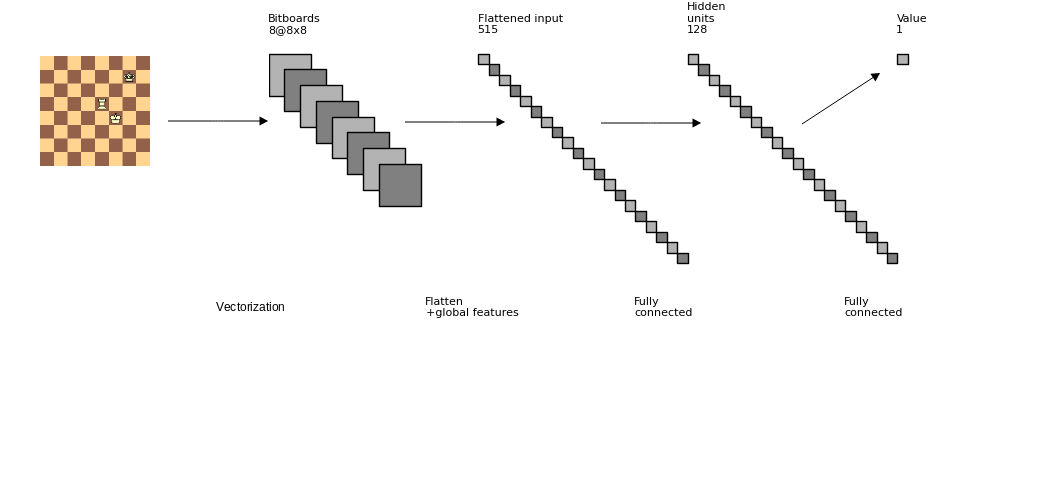
\includegraphics[trim={0 6cm 0 0cm},clip,scale=0.24]{arch/fc}
\subcaption{Depiction of the \gls{nn} used in the first experiment. The binary input features are fed into a 1 layer \gls{fnn}.}
\label{fig:fnn}
\end{subfigure}
\begin{subfigure}{0.4\textwidth}
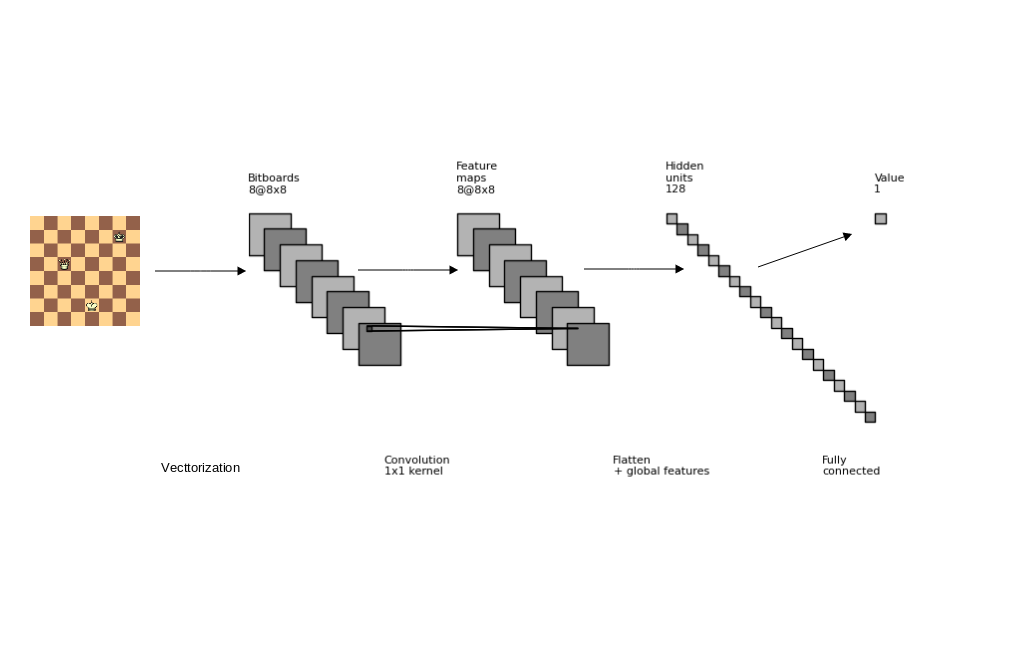
\includegraphics[trim={0 6cm 0 6cm},clip,scale=0.24]{arch/cnn1}
\subcaption{The (relatively simple) \gls{cnn} architecture deployed in experiment 2.}
\label{fig:cnn1}
\end{subfigure}
\caption{Network architectures used for the value function during the experiments.}
\end{figure}

\subsection{Experiment 1: king rook king endgame}
The first simulations we ran were on the \gls{krk} endgame, where the obvious goal for the player holding the rook is to checkmate the opponent as efficiently as possible. As only kings and rooks are set on the board, the input channels are limited to 8 bitboards. The network is trained with a learning rate of $\alpha=10^{-4}$, its architecture is represented in figure \ref{fig:fnn}. After every iteration during a stage, the exploration parameter $\epsilon$ is decreased according to the function $f_\epsilon(i)=(i)^{-3/4}$.\\
Table \ref{tab:perf_krk} confirms the hypothesis of TD-Stem being a faster learner than TD-Leaf. With the value function learned in TD-Stem, we succeed at winning about 85\% of the positions, clearly outperforming TD-Leaf. When the engine is at the losing side, it defends itself better with the novel variant.
\begin{table}[]
\centering
\caption{Performance comparison TD-Leaf($\lambda$) and TD-Stem($\lambda$),$N$ is the total number of episodes played in the simulation.}
\label{tab:perf_krk}
\begin{tabular}{l|rr}
    & \multicolumn{1}{l}{\textbf{TD-Leaf($\lambda$)}} & \multicolumn{1}{l}{ \textbf{TD-Stem($\lambda$)}} \\ \hline
\textbf{WCR} & 0.48                                   & \textbf{0.85}                          \\
\textbf{WE}  & \textbf{0.87}                          & 0.86                                   \\
\textbf{LHS} & 0.80                                   & \textbf{0.91}                          \\
\textbf{N }  & 353 500                                & \textbf{304 500}                      
\end{tabular}
\end{table}
\subsection{Experiment 2: king queen king endgame}
We try to confirm our conjecture of TD-Leaf being at least equivalent to TD-Stem in performance by analyzing an even easier problem, the \gls{kqk} endgame. The learning rate of the network depicted in figure \ref{fig:cnn1} is $\alpha=10^{-4}$. The exploration parameter $\epsilon$ obeys the decay function $f_{\epsilon}(i)=1-0.02i$.\\

A first glance at the learning curve in figure \ref{fig:lc_kqk} can trick one in believing that TD-Leaf learns quicker than TD-Stem. However, the sudden dive in the curve starting from episode 30000 corresponding with TD-Leaf hints to a contrary belief. An explanation for this behavior is that the winning rate in the plot represents the agents strength against itself, and not against the optimal agent. Hence, the decrease is a sign of an improvement at the losing side.\\
We can back this up with the observations noted in table \ref{tab:perf_kqk}, where we can see how both models still largely improve in the upcoming stages after the plateau in the learning curve is reached. Furthermore, TD-Stem plays stronger than TD-Leaf at the point in the plateau, confirming our belief of our proposal being the faster learner.\\

We provide two possible reasons why TD-Stem outperforms TD-Leaf in our experiments:
\begin{enumerate}
\item The influence of positive rewards propagates faster in updates, because depth plays a fundamental part to the learned value function at the states and their leaf nodes and so on.
\item The wrong belief effect in TD-Leaf slows down learning
\end{enumerate}
\begin{table}[]
\centering
\caption{Performance comparison TD-Leaf($\lambda$) and TD-Stem($\lambda$)}
\label{tab:perf_kqk}
\begin{tabular}{l|rr|rr}
& \multicolumn{2}{c|}{\textbf{3 stages}} & \multicolumn{2}{c}{\textbf{5 stages}} \\

    &\multicolumn{1}{l}{\small\textbf{TD-Leaf($\lambda$)}} & \multicolumn{1}{l|}{\small\textbf{TD-Stem($\lambda$)}}&\multicolumn{1}{l}{\small\textbf{TD-Leaf($\lambda$)}} & \multicolumn{1}{l}{\small\textbf{TD-Stem($\lambda$)}} \\ \hline
\textbf{WCR} & 0.65 & \textbf{0.77} & 0.90                                  & 0.90                          \\
\textbf{WE} & \textbf{0.67} & 0.64 & 0.89                          & 0.89                                   \\
\textbf{LHS} & 0.89 & 0.89 & 0.95                                   & \textbf{0.97}                          \\
\textbf{N } & \textbf{26000} & 27000  & \textbf{43500}                                & 44500                      
\end{tabular}
\end{table}

\begin{figure}
\centering
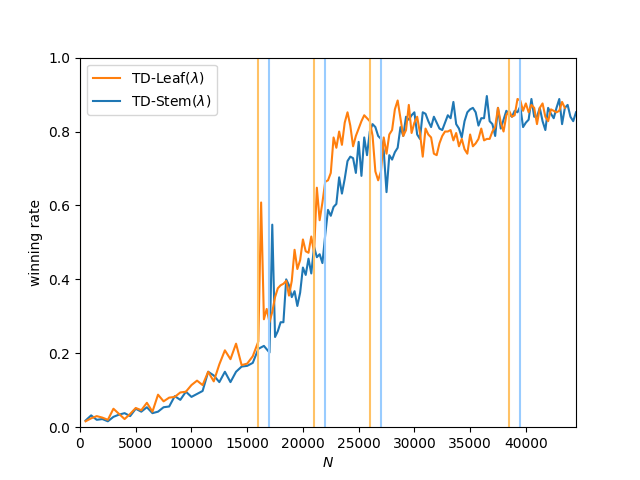
\includegraphics[scale=0.5]{plots/kqk_lc}
\caption{The learning curve of the second experiment, divided in 5 stages.}
\label{fig:lc_kqk}
\end{figure}

\section{Conclusion}
\label{sec:con}

In this study, a different approach from existing chess engines has been tried by not including any human bias to the system. To attain this property, only raw bitboard features and objective information about chess positions are fed into an \gls{nn}. The value function is learned through self play in combination with a novel \gls{rl} algorithm we called TD-Stem($\lambda$). We have compared this proposal with TD-Leaf($\lambda$) and the outcome of the experiments indicate that our variant learns faster.\\

More research can and needs to be carried out to obtain valuable knowledge about strategic game play in chess. Just as in backgammon, there might valuable positional knowledge in the game which has not been discovered yet. To explore these possibilities with \gls{rl} however, it is important to only make use of objective information (like tablebases for instance).\\

Possibilities to continue research are for example by learning on bigger endgame examples, deeper \glspl{cnn}, more bitboards extracted from chess positions and learning policy networks.

\nocite{*}
\bibliographystyle{phdsymp}
%%%%%\bibliography{bib-file}  % commented if *.bbl file included, as
%%%%%see below


%%%%%%%%%%%%%%%%% BIBLIOGRAPHY IN THE LaTeX file !!!!! %%%%%%%%%%%%%%%%%%%%%%%%
%% This is nothing else than the phdsymp_sample2e.bbl file that you would%%
%% obtain with BibTeX: you do not need to send around the *.bbl file        
%%
%%---------------------------------------------------------------------------%%
%
\begin{thebibliography}{1}
\bibitem{shannon}
Claude E. Shannon,
\newblock {\em Programming a computer for playing chess},
\newblock Philosophical Magazine, 41(314) 1950

\bibitem{turing}
Alan Turing,
\newblock {\em Chess},
\newblock Digital Computers applied to Games, 1953

\bibitem{deepblue}
Murray Campbell, Joseph Hoane Jr, Feng-hsiung Hsu 
\newblock {\em Deep Blue},
\newblock Artificial Intelligence, Vol. 134, p57-83, 2002

\bibitem{sota}
\newblock {\em CCRL 40/40 Rating List}
\newblock {\url{http://www.computerchess.org.uk/ccrl/4040/cgi/compare\_engines.cgi?print=Rating+list+%28text%29&class=all+engines&only_best_in_class=1}}
\newblock 2017

\bibitem{samuel}
Arthur L. Samuel 
\newblock {\em Some Studies in Machine Learning Using the Game of Checkers},
\newblock {IBM} Journal of Research and Development, Vol. 3, p210-229, 1959

\bibitem{tesauro}
Gerald Tesauro
\newblock {\em Temporal Difference Learning and TD-Gammon},
\newblock Communications of the ACM, Vol. 38, p58-68, 1995

\bibitem{knightcap}
Jonathan Baxter, Andrew Tridgell and Lex Weaver
\newblock {\em TDLeaf(lambda): Combining Temporal Difference Learning with Game-Tree Search},
\newblock CoRR, 1999

\bibitem{giraffe}
Matthew Lai
\newblock {\em Giraffe: Using Deep Reinforcement Learning to Play Chess},
\newblock diploma thesis Imperial College London, 2015

\bibitem{meep}
Joel Veness, David Silver, Alan Blair and William Uther
\newblock {\em Bootstrapping from Game Tree Search},
\newblock Advances in Neural Information Processing System Vol. 22 p.1937-1945, 2009

\bibitem{deepchess}
Omid E. David, Nathan S. Netanyahu, Lior Wolf
\newblock {\em DeepChess: End-to-End Deep Neural Network for Automatic Learning in Chess},
\newblock Artificial Neural Networks and Machine Learning – ICANN 2016

\bibitem{atari}
Volodymyr Mnih, Koray Kavukcuoglu, David Silver, Alex Graves, Ioannis Antonoglou, Daan Wierstra and Martin Riedmiller
\newblock {\em Playing Atari with Deep Reinforcement Learning},
\newblock NIPS Deep Learning Workshop 2013

\bibitem{dddqn}
Ziyu Wang, Nando de Freitas and Marc Lanctot
\newblock {\em Dueling Network Architectures for Deep Reinforcement Learning},
\newblock CoRR 2015

\bibitem{alphago}
David Silver, Aja Huang, Chris J. Madison et al.
\newblock {\em Mastering the game of Go with deep neural networks and tree search},
\newblock Nature Vol. 529 p484-489, 2016


\bibitem{rl}
Richard S. Sutton and Andrew G. Barton,
\newblock {\em Introduction to Reinforcement Learning},
\newblock 1998

\bibitem{alphabeta}
George T. Heineman, Gary Pollice andStanley Selkow (2008),
\newblock {\em Algorithms in a Nutshell},
\newblock p217–223, 1998

\bibitem{rlalg}
Csaba Szepesv{\'a}ri
\newblock {\em Algorithms for Reinforcement Learning},
\newblock 2010

\bibitem{convergence}
J.N. Tsitsikilis, B.V. Roy 
\newblock{\em An Analysis of Temporal Difference Learning with Function Approximation }
\newblock IEEE Transactions on Automatic Control, Vol.42(5), p674–690 1996

\bibitem{tb}
Galen Huntington, Guy Haworth, 
\newblock{\em Depth to Mate and the 50-Move Rule.}
\newblock ICGA Journal, Vol. 38, No. 2

\bibitem{init}
Xavier Glorot, Yoshua Bengio
\newblock{\em Understanding the difficulty of training deep feedforward neural networks}
\newblock Proceedings of the Thirteenth International Conference on Artificial Intelligence and Statistics, PMLR 9: p249-256, 2010

\end{thebibliography}
%
%%---------------------------------------------------------------------------%%



\end{document}

%%%%%%%%%%%%%%%%%%%%%  End of phdsymp_sample2e.tex  %%%%%%%%%%%%%%%%%%%%%%%%%%%
